
\documentclass[12pt]{exam}
\usepackage{amsthm}
\usepackage{libertine}
%\usepackage[utf8]{inputenc}
\usepackage[margin=1in]{geometry}
\usepackage{amsmath,amssymb}
\usepackage{multicol}
\usepackage[shortlabels]{enumitem}
\usepackage{siunitx}
\usepackage{cancel}
\usepackage{graphicx}
\graphicspath{{./}}
\usepackage{pgfplots}
\usepackage{hyperref}
\usepackage{listings}
\usepackage{tikz}
\usepackage{minted}
\def\code#1{\texttt{#1}}
\usepackage{amssymb}
\usepackage{xcolor}
% for plotting
\usepackage{pgfplots}
\pgfplotsset{compat=1.16}
\usepackage{tikz}
\usetikzlibrary{arrows.meta}

\newcommand{\quotebox}[1]
{
  \begin{center}
    \fcolorbox{white}{blue!15!gray!15}{
      \begin{minipage}{0.7\linewidth}\vspace{10pt}
        \center
        \begin{minipage}{0.8\linewidth}{\space\Huge``}{\setlength{\parindent}{1.5em}#1}{\hspace{1.5em}\break\null\Huge\hfill''}
        \end{minipage}
        \smallbreak
      \end{minipage}
    }
\end{center}
}

% for plotting half circle
% call it with \MyHalfCircle{<size>}{<x coord>}{<y coord>} in tikz pictur
\newcommand{\MyHalfCircle}[3][0.4ex]{%
    % #1 = size
    % #2 = x coordinate
    % #3 = y coordinate
  \begin{scope}
   \draw (axis cs:#2,#3) circle (#1);
   \clip (axis cs:#2,#3) circle (#1);
   \fill[red, opacity=0.75] (axis cs:#2,#1) rectangle (axis cs:-#1,-#1);
  \end{scope}
}

%\DeclareUnicodeCharacter{2212}{-}


\let\oldemptyset\emptyset
\let\emptyset\varnothing

\hypersetup{
    colorlinks=true,
    linkcolor=blue,
    filecolor=magenta,      
    urlcolor=cyan,
    pdftitle={Overleaf Example},
    pdfpagemode=FullScreen,
    }
    
\urlstyle{same}

\pgfplotsset{width=10cm,compat=1.9}
\usepgfplotslibrary{external}
\tikzexternalize

\newcommand{\class}{Math 415} % This is the name of the course 
\newcommand{\examnum}{Homework-2} % This is the name of the assignment
\newcommand{\examdate}{September 21} % This is the due date
\newcommand{\timelimit}{}

\newcommand{\BO}{\mathcal{O}}




\begin{document}
\pagestyle{plain}
\thispagestyle{empty}

\noindent
\begin{tabular*}{\textwidth}{l @{\extracolsep{\fill}} r @{\extracolsep{6pt}} l}
\textbf{\class} & \textbf{Name:} & \textit{Zhenzhao Tu}\\ %Your name here instead, obviously 
\textbf{\examnum} &&\\
\textbf{\examdate} &&\\
\end{tabular*}\\
\rule[2ex]{\textwidth}{2pt}
% --


\section*{Problem 1}
The vector field of \(x' = ax^2\) is right and check below:

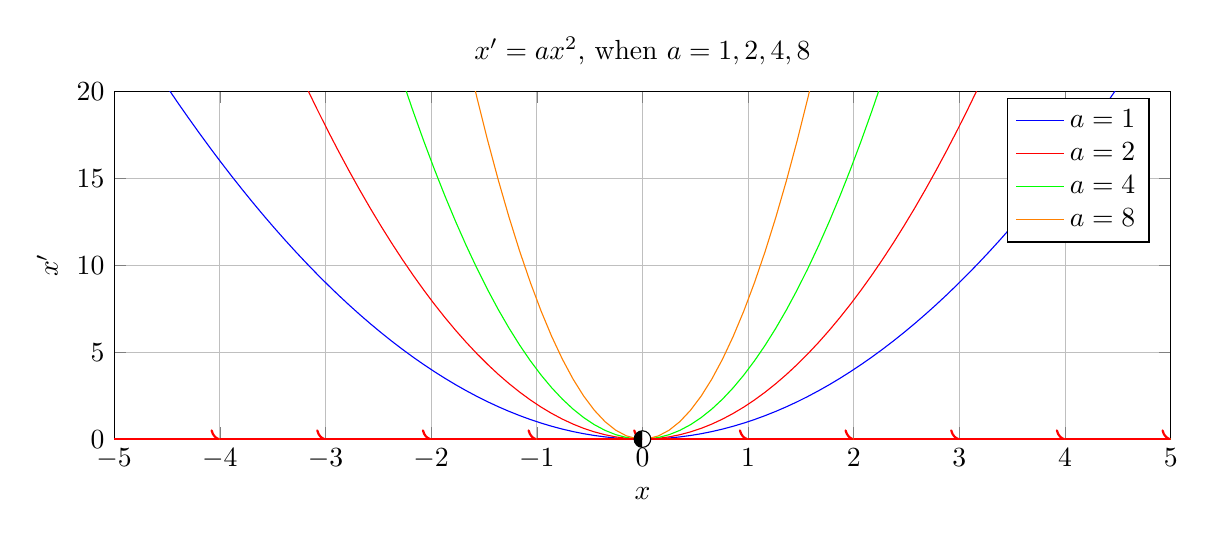
\begin{tikzpicture}
	\begin{axis}[
		title={\(x' = ax^2\), \text{when} \(a = 1, 2, 4, 8\)},
		xlabel={\(x\)},
		ylabel={\(x'\)},
		xmin=-5, xmax=5,
		ymin=0, ymax=20,
		grid=major,
		width=15cm,
		height=6cm,
	]
	% when a = 1
	\addplot[blue, domain=-5:5, samples=100] {x^2};
	% when a = 2
	\addplot[red, domain=-5:5, samples=100] {2*x^2};
	% when a = 4
	\addplot[green, domain=-5:5, samples=100] {4*x^2};
	% when a = 8
	\addplot[orange, domain=-5:5, samples=100] {8*x^2};
	% horizontal lines at 0
	\addplot[orange, thick, domain=-5:5, samples=100] {0};

	% add a half circle at (0, 0)
	\addplot[mark=halfcircle*, mark options={rotate=90}, mark size=3pt] coordinates {(0, 0)};
	
	% draw vector at (-5, 0) toword (-4,0) and change the size of the arrow
	\addplot[->, thick, color=red] coordinates {(-5,0) (-4,0)};
	% draw vector at (-4, 0) toword (-3,0)
	\addplot[->, thick, color=red] coordinates {(-4,0) (-3,0)};
	% draw vector at (-3, 0) toword (-2,0)
	\addplot[->, thick, color=red] coordinates {(-3,0) (-2,0)};
	% draw vector at (-2, 0) toword (-1,0)
	\addplot[->, thick, color=red] coordinates {(-2,0) (-1,0)};
	% draw vector at (-1, 0) toword (0,0)
	\addplot[->, thick, color=red] coordinates {(-1,0) (0,0)};
	% draw vector at (0, 0) toword (1,0)
	\addplot[->, thick, color=red] coordinates {(0,0) (1,0)};
	% draw vector at (1, 0) toword (2,0)
	\addplot[->, thick, color=red] coordinates {(1,0) (2,0)};
	% draw vector at (2, 0) toword (3,0)
	\addplot[->, thick, color=red] coordinates {(2,0) (3,0)};
	% draw vector at (3, 0) toword (4,0)
	\addplot[->, thick, color=red] coordinates {(3,0) (4,0)};
	% draw vector at (4, 0) toword (5,0)
	\addplot[->, thick, color=red] coordinates {(4,0) (5,0)};

	\legend{\(a = 1\), \(a = 2\), \(a = 4\), \(a = 8\)}
	\end{axis}
\end{tikzpicture}
\\
Also, the vector field of \(x' = -ax^2\) is below:
\\
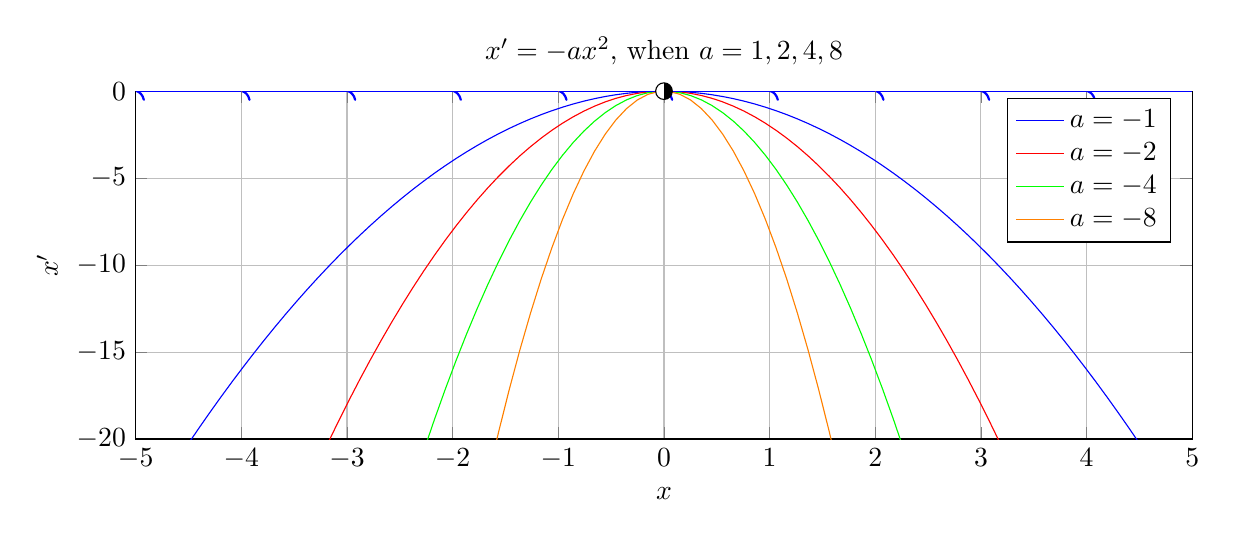
\begin{tikzpicture}
	\begin{axis}[
		title={\(x' = -ax^2\), \text{when} \(a = 1, 2, 4, 8\)},
		xlabel={\(x\)},
		ylabel={\(x'\)},
		xmin=-5, xmax=5,
		ymin=-20, ymax=0,
		grid=major,
		width=15cm,
		height=6cm,
	]
	% when a = -1
	\addplot[blue, domain=-5:5, samples=100] {-x^2};
	% when a = -2
	\addplot[red, domain=-5:5, samples=100] {-2*x^2};
	% when a = -4
	\addplot[green, domain=-5:5, samples=100] {-4*x^2};
	% when a = -8
	\addplot[orange, domain=-5:5, samples=100] {-8*x^2};
	% horizontal lines at 0
	\addplot[orange, thick, domain=-5:5, samples=100] {0};
	
	% add a half circle at (0, 0)
	\addplot[mark=halfcircle*, mark options={rotate=-90}, mark size=3pt] coordinates {(0, 0)};
	
	% draw vector at (5, 0) toword (4,0) and change the size of the arrow
	\addplot[->, thick, color=blue] coordinates {(5,0) (4,0)};
	% draw vector at (4, 0) toword (3,0)
	\addplot[->, thick, color=blue] coordinates {(4,0) (3,0)};
	% draw vector at (3, 0) toword (2,0)
	\addplot[->, thick, color=blue] coordinates {(3,0) (2,0)};
	% draw vector at (2, 0) toword (1,0)
	\addplot[->, thick, color=blue] coordinates {(2,0) (1,0)};
	% draw vector at (1, 0) toword (0,0)
	\addplot[->, thick, color=blue] coordinates {(1,0) (0,0)};
	% draw vector at (0, 0) toword (-1,0)
	\addplot[->, thick, color=blue] coordinates {(0,0) (-1,0)};
	% draw vector at (-1, 0) toword (-2,0)
	\addplot[->, thick, color=blue] coordinates {(-1,0) (-2,0)};
	% draw vector at (-2, 0) toword (-3,0)
	\addplot[->, thick, color=blue] coordinates {(-2,0) (-3,0)};
	% draw vector at (-3, 0) toword (-4,0)
	\addplot[->, thick, color=blue] coordinates {(-3,0) (-4,0)};
	% draw vector at (-4, 0) toword (-5,0)
	\addplot[->, thick, color=blue] coordinates {(-4,0) (-5,0)};

	\legend{\(a = -1\), \(a = -2\), \(a = -4\), \(a = -8\)}
	\end{axis}
\end{tikzpicture}

Discussion: When \(a > 0\), the vector field is pointing to the right, and when \(a < 0\), the vector field is pointing to the left. That indicates both cases are half-stable. However the different between these two cases are the $x(t)$ is increasing when $a > 0$ and $x(t)$ is decreasing when $a < 0$.

\newpage
\section*{Problem 2}
\begin{enumerate}
	\item Let $x(t) = x^* + \eta(t)$, with $\eta \ll x^*$ and $f(x^*) = f'(x^*) = 0$. Then we have
		\[\eta(t) = x(t) - x^*\]
	when we take derivative on both sides, we have
		\[\frac{d}{dt}\eta(t) = \frac{d}{dt}x(t) - \frac{d}{dt}x^*\]
	since $x'=f(x)$, we have
		\[\frac{d}{dt}\eta(t) = f(x) - f(x^*).\]
	So, by replacing $x$ with $x^* + \eta(t)$, we have
		\[\eta'(t) = f(x^* + \eta(t)) - 0.\]
	Now, if we using Talyar Expension on $f(x^* + \eta(t))$, we have
		\[f(x^* + \eta(t)) = f(x^*) + f'(x^*)\eta(t) + \frac{1}{2}f''(x^*)\eta^2(t) + \BO(\eta^3(t)).\]
	Since $f(x^*) = f'(x^*) = 0$ and $\BO(\eta^3(t))$ is negligible, we have
		\[\eta'(t) \approx \frac{1}{2}f''(x^*)\eta^2(t).\]

	\item In Q1 cases, the $f''(x^*) = 2a$, so the $\eta'(t) = a\eta^2(t)$. When $a > 0$, $\eta'(t) > 0$, which means $\eta(t)$ is increasing qadratically. And when $a < 0$, $\eta'(t) < 0$, which means $\eta(t)$ is decreasing qadratically. So, $x=x^*$ is unstable when $a > 0$ and it is stable when $a < 0$.
	
\end{enumerate}

\section*{Problem 3}
For $x'=ax-x^3$, we will going to use Linear Stability Analysis to discuss fixed point when $a > 0$ and $a < 0$.

Let $x^*$ be a fixed point, and let $x(t) = x^* + \eta(t)$, with $\eta \ll x^*$ and $f(x^*) = f'(x^*) = 0$. Then we have
	\[\eta(t) = x(t) - x^*.\]
By Q2(a) step, we can finally get approximate equation
	\[\eta'(t) \approx f'(x^*)\eta(t).\]
So, in our case we have
	\[\eta'(t) \approx (a - 3x^{*2})\eta(t).\]
The fixed point occurs when $ax-x^3 = 0$. Thus $x^*=0$ and $x^*=\pm\sqrt{a}$ are fixed points. When $a > 0$, we have $x^*=\pm\sqrt{a}$ are fixed points. And when $a < 0$, we have $x^*=0$ is the only fixed point. So, we will discuss these two cases separately.
Then, when $a > 0$, we have
\[ f'(x^*) = a - 3x^{*2} =
\begin{cases}
	-2a & \text{when } x^* = \sqrt{a} \\
	-2a & \text{when } x^* = -\sqrt{a} \\
	a & \text{when } x^* = 0
\end{cases}
\]
That indicate $x^* = \sqrt{a}$ is stable, $x^* = -\sqrt{a}$ is stable, and $x^* = 0$ is unstable.

When $a < 0$, we have
\[ f'(x^*) = a - 3x^{*2} = a \quad \text{when } x^*=0\]
That indicate $x^* = 0$ is stable at $a < 0$.


\section*{Problem 4}
The height of the water in bucket is $h(t)$, and the IVP is 
\[h' = -Q \sqrt{h}, \quad h(0) = h_0.\]

\begin{enumerate}[(a)]
	\item The solution of the IVP is below:
	Divide both sides by $\sqrt{h}$, we have
	\[\frac{h'}{\sqrt{h}} = -Q.\]
	Integrate both sides respect to $t$, we have
	\[\int \frac{\frac{h'}{dt}}{\sqrt{h}} dt = \int -Q dt.\]
	Evaluate the integral, we have
	\[2\sqrt{h} = -Qt + C.\]
	Plug in the initial condition, we have
	\[h(t) = \frac{1}{4}(-Qt + C)^2.\]
	Since $h(0)=h_0$, we have
	\[C = 2\sqrt{h_0}.\]
	So, the solution of the IVP is
	\[h(t) = \frac{1}{4}(-Qt + 2\sqrt{h_0})^2.\]

	\item Let $h(t) = 0$, we can find the time when the bucket is empty. So, we have
	\[0 = \frac{1}{4}(-Qt + 2\sqrt{h_0})^2.\]
	That means $t = \frac{2\sqrt{h_0}}{Q}$. So, the time when the bucket is empty is $\frac{2\sqrt{h_0}}{Q}$.

	\item The bucket is full when $h(t) = H$. So, we have
	\[H = \frac{1}{4}(-Qt + 2\sqrt{h_0})^2.\]
	That means $t = \frac{2\sqrt{h_0}}{Q} - \frac{2\sqrt{H}}{Q}$. So, the time when the bucket is full is $\frac{2\sqrt{h_0}}{Q} - \frac{2\sqrt{H}}{Q}$.

	\item If $h_0=0$, then we have solution
		\[h(t) = \frac{1}{4}(-Qt)^2 = \frac{1}{4}Q^2t^2.\]
		Even for $t \leq 0$, the height of the water is always non-negative.
	However, it is obverse that $h(t)=0$ is also a solution when $h_0=0$, since the height of the water is always zero if the initial height is zero. So, show that the solution is not unique when $h_0=0$.

	\item When the initial value $h_0=0$, the solution is not unique. That means if we think of reverse time $(t \leq 0)$, it has infinite possible situation could happend. In physical, it is possible that water is always empty or it could be has water at sometime past and then empty at sometime later. So, the reverse time is not unique when $h_0=0$.

\end{enumerate}

\section*{Problem 5}
The potential function $V(x)$ for $x' = -2x \cos(x^2)$ is below:
\[V(x) = \int 2x \cos(x^2) dx = \sin(x^2) + C.\]
Then the plot of $V(x)$ is below (when $C=0$):

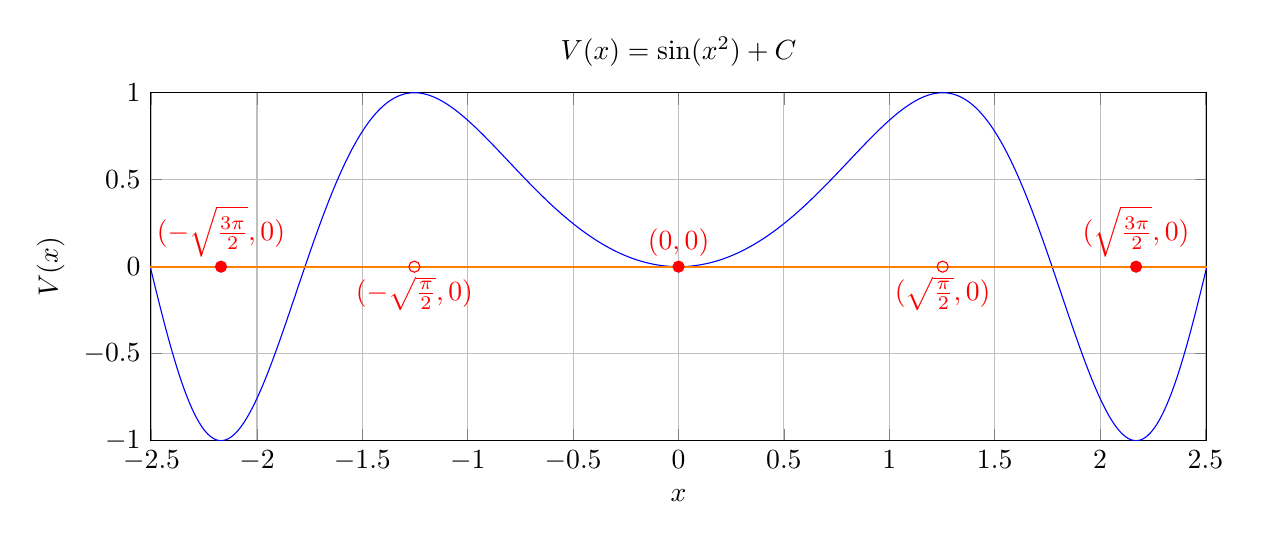
\begin{tikzpicture}
	\begin{axis}[
		title={\(V(x) = \sin(x^2) + C\)},
		xlabel={\(x\)},
		ylabel={\(V(x)\)},
		xmin=-sqrt(2*pi), xmax=sqrt(2*pi),
		ymin=-1, ymax=1,
		grid=major,
		width=15cm,
		height=6cm,
	]
	% when C = 0
	\addplot[blue, domain=-sqrt(2*pi):sqrt(2*pi), samples=700] {sin(deg(x^2))};
	% horizontal lines at 0
	\addplot[orange, thick, domain=-sqrt(2*pi):sqrt(2*pi), samples=100] {0};
	% add thick dash line at x=\sqrt(2\pi) and label it
	% \addplot[thick, dashed, color=red] coordinates {({sqrt(2*pi)}, 1) ({sqrt(2*pi)}, -1)};
	% add thick dash line at x=-\sqrt(2\pi) and label it
	% \addplot[thick, dashed, color=red] coordinates {({-sqrt(2*pi)}, 1) ({-sqrt(2*pi)}, -1)};

	% add a point at (0, 0) and label it
	\addplot[only marks, mark=*, mark size=2pt, color=red] coordinates {(0, 0)} node[anchor=south] {\((0, 0)\)};
	% add a hollow point at (\sqrt(\pi/2), 0) and label it
	\addplot[only marks, mark=o, mark size=2pt, color=red] coordinates {({sqrt(pi/2)}, 0)} node[anchor=north] {\((\sqrt{\frac{\pi}{2}}, 0)\)};
	% add a hollow point at (-\sqrt(\pi/2), 0) and label it
	\addplot[only marks, mark=o, mark size=2pt, color=red] coordinates {({-sqrt(pi/2)}, 0)} node[anchor=north] {\((-\sqrt{\frac{\pi}{2}}, 0)\)};
	% add a point at (\sqrt(3\pi/2), 0) and label it
	\addplot[only marks, mark=*, mark size=2pt, color=red] coordinates {({sqrt(3*pi/2)}, 0)} node[anchor=south] {\((\sqrt{\frac{3\pi}{2}}, 0)\)};
	% add a point at (-\sqrt(3\pi/2), 0) and label it
	\addplot[only marks, mark=*, mark size=2pt, color=red] coordinates {({-sqrt(3*pi/2)}, 0)} node[anchor=south] {\((-\sqrt{\frac{3\pi}{2}}, 0)\)};


	\end{axis}
\end{tikzpicture}

By solving $x'=0$, we have fixed points $x^* = \pm \sqrt{\frac{\pi}{2}+k\pi}$ where $k \in \{0, 1\}$.

Now we know the stability of $V(x)$ in $[-\sqrt{2\pi}, \sqrt{2\pi}]$ can be read from the plot. The $x^* = \pm \sqrt{\frac{\pi}{2}}$ are unstable, while the $x^*=0$ and $x^* = \pm \sqrt{\frac{3\pi}{2}}$ are stable.




\end{document}

